\chapter{Analisi dei Requisiti}

\section{Obiettivi del sistema}


\begin{itemize}
\item progettazione e implementazione dei vari codec in un formato mdc-compatibile
\item progettazione e implementazione di un protocollo per lo scambio dei
flussi di dati in modo \emph{peer-to-peer} (chiamato MDSP)
\item piattaforma per il test dell'insieme
\end{itemize}


\section{Codifica}


Un \emph{codec} è un dispositivo (hardware o software) in grado di codificare e
decodificare alcune informazioni in un formato di rappresentazione particolare.
In genere il termine è usato in relazione a flussi multimediali (audio/video)
processati tramite un elaboratore elettronico.
Esistono molti modelli per la realizzazione di codec: u


\subsection{Modello \emph{Layered}}
Il Modello \emph{Layered} prevede che i codec debbano suddividere un flusso
multimediale in:
\begin{itemize}
  \item uno ``strato base'' (\emph{Base Layer})
  \item diversi ``strati di avanzamento'' (\emph{Enhancement Layers}) 
\end{itemize}

Il principio è che gli \emph{Enhancement Layers}, essendo non necessari, possano
essere inviati solo a chi ne fa specifica richiesta, per aumentare la
qualità del flusso.

Questo tipo di approccio, anche se molto diffuso\footnote{Il Modello
\emph{Layered} è alla base di codec come MPEG e derivati (MP3, DivX, ecc.)},
presenta alcune problematiche.

I flussi multimediali generalmente vengono trasmessi tramite reti che non
garantiscono il trasporto privo di errori (\emph{best effort}). Ogni pacchetto
inviato ha una certa probabilità di giungere a destinazione corrotto, oppure di
non arrivare affatto. Nel Modello \emph{Layered} questi errori potrebbero
intaccare in pacchetto di un \emph{Enhancement Layer} oppure di un \emph{Base
Layer}: nel primo caso si avrà solo una piccola perdita di qualità, mentre nel
secondo caso si avranno conseguenze potenzialmente disastrose, come la perdita
di continuità nel flusso. Se il flusso non è real-time, è possibile chiedere
nuovamente alla sorgente il frammento danneggiato: un \emph{Base Layer} però
contiene solitamente molte più informazioni, quindi è più oneroso
ritrasmetterlo.
Infine, gli \emph{Enhanchement Layers} hanno un senso solo se rapportati al
loro strato base, quindi è necessario far si che giungano in istanti di
tempo vicini: altrimenti sarebbero inutili.


%TODO: inserire immagine sul modello layered

\subsection{Modello \emph{Multiple Descriptions}}

Il Multiple Description Coding prevede che:
\begin{enumerate}
\item il flusso informativo sia suddiviso in più frammenti, detti 'Descrittori', con circa la stessa quantità di informazioni
\item i descrittori costituiscano due o più sotto-flussi;
\item i descrittori di un solo sotto-flusso, qualunque sia, devono bastare a ricostruire l'informazione, per lo meno con una bassa qualità
\item se vengono ricevuti due o più sotto-flussi, la qualità dell'informazione decodificata aumenta 
\end{enumerate}

TODO: inserire immagine sul modello mdc

\subsection{Differenze tra MDC e Layered}

La principale differenza tra la tipologia di codifica 'a descrizioni multiple' e
quella 'a strati' sta nella differente organizzazione delle informazioni: i
frammenti ottenuti con una codifica MDC hanno potenzialmente lo stesso contenuto
informativo in termini di quantità, mentre nei codec 'layered' esiste un
frammento 'base', più importante degli altri, e diversi frammenti più piccoli di
'avanzamento'.






\section{Testbed}



\subsection{Organizzazione}


Il testbed è composto da un insieme di classi, suddivise per tipologia:



\begin{itemize}
\item \emph{common}: classi che facilitano la realizzazione delle proprie
applicazioni; comprendono utility per accedere alla rete, per simulare un comportamento multi-tasking, e altro.

\item \emph{codecs}: contiene sia classi astratte, da usare come base per i
codec reali, sia classi di utilità, come il registro dei codec, utilizzato per auto-caricare il codec adatto a seconda del flusso informativo

\item \emph{messages}: l'insieme dei messagi di base
\item \emph{app}: una applicazione client-server di esempio
\end{itemize}




\subsection{Implementazione}


Il testbed è stato sviluppato in C/C++, anche se, seguendo le specifiche, è
possibile implementare una qualunque parte del sistema con qualsiasi linguaggio.

\`E stato sviluppato un client in python.



\section{MDSP}


MDSP sta per Multiple Description Stream Protocol, ed è un protocollo per lo
scambio di stream di vario tipo (contenuti multimediali) organizzati secondo una
meta-codifica a descrittori multipli.

\begin{figure}[hb]
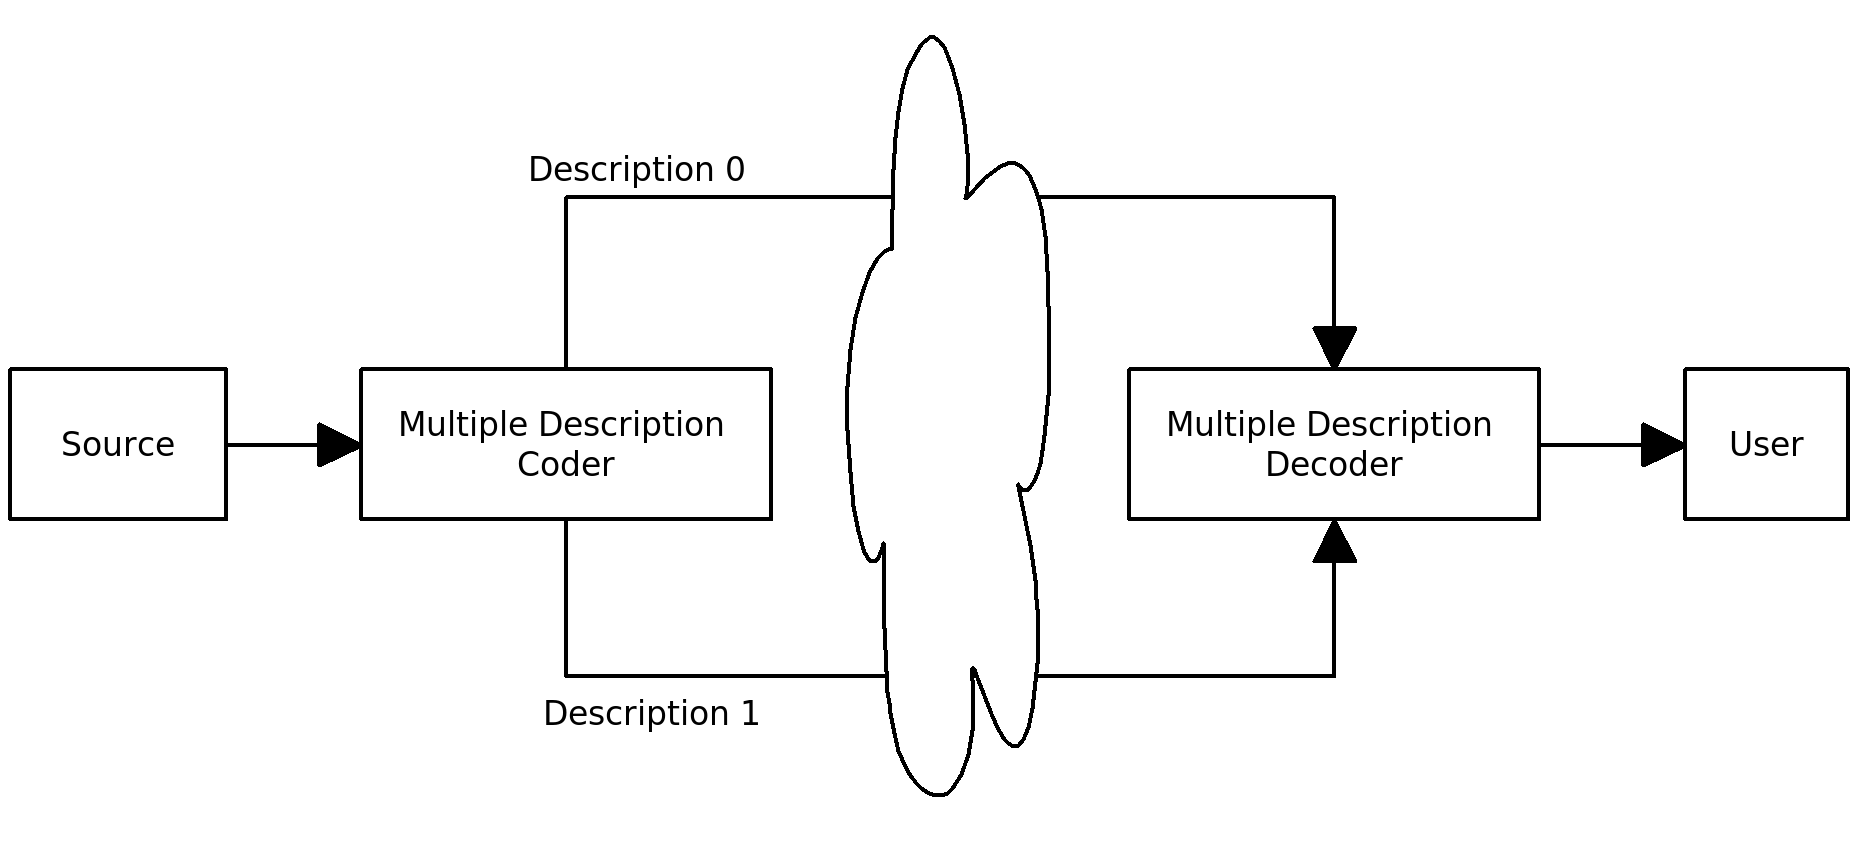
\includegraphics[width=0.90\textwidth]{../images/network_mdc.png}
\label{fig:network_mdc}
\caption{Modello di rete basata su MDC}
\end{figure}

Tale protocollo è concepito per avere le seguenti caratteristiche:
\begin{itemize}
  \item ogni messaggio è indipendente dagli altri
  \item nessuna ritrasmissione dei messaggi errati o mancanti
  \item nessun tipo di controllo di errore
  \item nessun tipo di controllo di flusso 
\end{itemize}

Le ultime tre caratteristiche, se necessarie, possono essere gestite a livelli
più alti dello stack protocollare.



\subsection{Canali}
Devono essere previsti ``canali'' per il trasporto di due tipi di informazioni:
\begin{itemize}
  \item \emph{messaggi di controllo}: per la gestione della rete
  \item \emph{dati}: i contenuti scambiati dagli utenti
\end{itemize}









